\documentclass[12pt]{article}
\usepackage{amsmath}
\usepackage{amssymb}
\usepackage{tikz}
\usepackage[margin=1in]{geometry}
\usepackage{graphicx}
\usepackage[colorlinks=true, linkcolor=blue, bookmarks=true, bookmarksopen=true]{hyperref}
\usepackage{blkarray}
\usepackage{float}

\usetikzlibrary{positioning}
\title{Module 2}
\begin{document}
\maketitle
\section{Channel Capacity}
The channel capacity of a discrete memory-less source is defined as the maximum mutual information $I(X,Y)$ in a channel. 
The channel capacity is measured in bits/channel used. 
$$C = \max [ I(X,Y) ]$$ 
The various channels used in communication systems are described below: 

\subsection{Lossless Channel}
A channel is said to be lossless if $H(X|Y) = 0$ for all distributions. 
A lossless channel is determined by the factor that the input is determined by the output and hence no transmission error can occur. 

\begin{minipage}{.4\linewidth}
$$\text{E.g: } P(Y|X) = \begin{blockarray}{cccccc}
 & y_1 & y_2 & y_3 & y_4 & y_5 \\
\begin{block}{c[ccccc]}
x_1 & 3/4 & 1/4 & 0 & 0 & 0 \\ 
x_2 & 0 & 0 & 1/3 & 2/3 & 0 \\ 
x_3 & 0 & 0 & 0 & 0 & 1 \\
\end{block}
\end{blockarray}$$
\end{minipage}%
\hfill
\begin{minipage}{.3\linewidth}
\centering
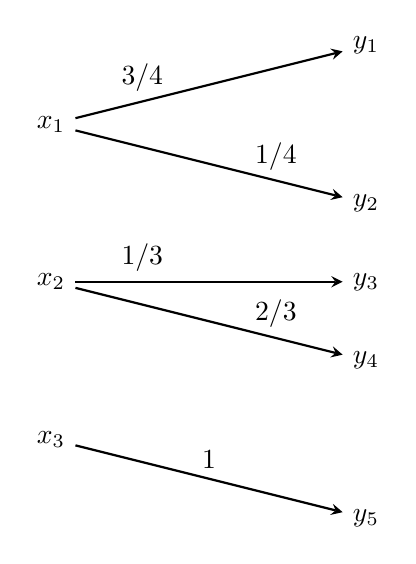
\begin{tikzpicture}[>=stealth, thick]
    \node (x1) at (0, 2) {$x_1$};
    \node (x2) at (0, 0) {$x_2$};
    \node (x3) at (0, -2) {$x_3$};

    \node (y1) at (4, 3) {$y_1$};
    \node (y2) at (4, 1) {$y_2$};
    \node (y3) at (4, 0) {$y_3$};
    \node (y4) at (4, -1) {$y_4$};
    \node (y5) at (4, -3) {$y_5$};

    \draw[->] (x1) -- node[above, near start] {3/4} (y1);
    \draw[->] (x1) -- node[above, near end] {1/4} (y2);
    \draw[->] (x2) -- node[above, near start] {1/3} (y3);
    \draw[->] (x2) -- node[above, near end] {2/3} (y4);
    \draw[->] (x3) -- node[above] {1} (y5);
\end{tikzpicture}
Equivalent representation
\end{minipage}
\subsubsection{Channel Capacity of A Lossless Channel}
We know that channel capacity = Max [Mutual Information] = $\max [I(X,Y)]$ 
$$I(X,Y) = H(X) - H(X|Y)$$ 
For a lossless channel $H(X|Y) = 0$ 
\begin{align*}
\therefore C &= \max [I(X,Y)] \\
&= \max [H(X) - 0] \\
&= \max [H(X)]
\end{align*} 
If the source is transmitting 'M' symbols the entropy will be maximum if all the signals are equally likely. Then the entropy $H = \log_2 M$ 
\begin{align*}
\therefore C &= \max [H(X)] \\
&= \log_2 M
\end{align*} 

\subsection{Deterministic Channel}
A channel is said to be deterministic if $P(Y|X) = 1$ equivalently $H(Y|X) = 0$ for all the index variable involved and for all input distributions. 
In the case of a deterministic channel the noise matrix contain only one non zero element in the row. The element is unity.

\begin{minipage}{.3\linewidth}
$$\text{E.g: } P(Y|X) = \begin{blockarray}{cccc}
 & y_1 & y_2 & y_3 \\
\begin{block}{c[ccc]}
x_1 & 1 & 0 & 0 \\ 
x_2 & 1 & 0 & 0 \\ 
x_3 & 0 & 1 & 0 \\ 
x_4 & 0 & 1 & 0 \\ 
x_5 & 0 & 0 & 1 \\
\end{block}
\end{blockarray}$$
\end{minipage}%
\hfill
\begin{minipage}{.5\linewidth}
\centering
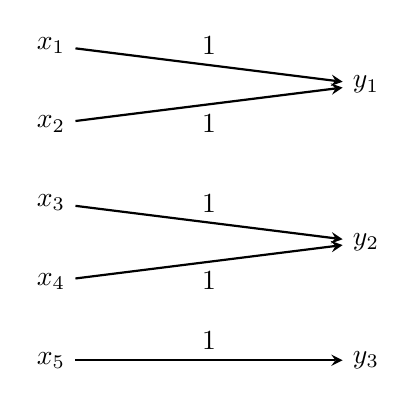
\begin{tikzpicture}[>=stealth, thick]
    \node (x1) at (0, 2) {$x_1$};
    \node (x2) at (0, 1) {$x_2$};
    \node (x3) at (0, 0) {$x_3$};
    \node (x4) at (0, -1) {$x_4$};
    \node (x5) at (0, -2) {$x_5$};
    
    \node (y1) at (4, 1.5) {$y_1$};
    \node (y2) at (4, -0.5) {$y_2$};
    \node (y3) at (4, -2) {$y_3$};
    
    \draw[->] (x1) -- node[above] {1} (y1);
    \draw[->] (x2) -- node[below] {1} (y1);
    \draw[->] (x3) -- node[above] {1} (y2);
    \draw[->] (x4) -- node[below] {1} (y2);
    \draw[->] (x5) -- node[above] {1} (y3);
\end{tikzpicture}
\end{minipage}

\subsubsection{Channel Capacity of A Deterministic Channel}
We know that channel capacity = Max [Mutual Information] = $\max [I(X,Y)]$ 
$$I(X,Y) = H(Y) - H(Y|X)$$ 
For a deterministic channel $H(Y|X) = 0$ 
$$\therefore C = \max [H(Y)]$$ 
If the receiver is receiving 'N' symbols the entropy will be maximum if all the signals are equally likely. Then the entropy $H = \log_2 N$ 
\begin{align*}
\therefore C &= \max [H(Y)] \\
&= \log_2 N
\end{align*} 

\subsection{Noiseless/Ideal Channel}
A channel is said to be noiseless if the channel is both lossless and deterministic. That is $H(Y|X) = H(X|Y) = 0$. 
That is the noise matrix contains a non zero entry in each row and each column. 

\begin{minipage}{.3\linewidth}
$$\text{E.g: } P(Y|X) = \begin{blockarray}{cccc}
 & y_1 & y_2 & y_3 \\
\begin{block}{c[ccc]}
x_1 & 1 & 0 & 0 \\ 
x_2 & 0 & 1 & 0 \\ 
x_3 & 0 & 0 & 1 \\
\end{block}
\end{blockarray}$$
\end{minipage}%
\hfill
\begin{minipage}{.5\linewidth}
\centering
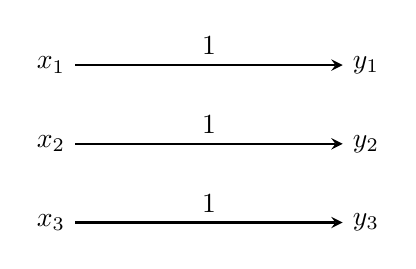
\begin{tikzpicture}[>=stealth, thick]
    \node (x1) at (0, 1) {$x_1$};
    \node (x2) at (0, 0) {$x_2$};
    \node (x3) at (0, -1) {$x_3$};
    
    \node (y1) at (4, 1) {$y_1$};
    \node (y2) at (4, 0) {$y_2$};
    \node (y3) at (4, -1) {$y_3$};
    
    \draw[->] (x1) -- node[above] {1} (y1);
    \draw[->] (x2) -- node[above] {1} (y2);
    \draw[->] (x3) -- node[above] {1} (y3);
\end{tikzpicture}
\end{minipage}

\subsubsection{Channel Capacity of A Noiseless Channel}
We know that channel capacity = Max [Mutual Information] = $\max [I(X,Y)]$ 
$$I(X,Y) = H(Y) - H(Y|X) = H(X) - H(X|Y)$$ 
For a noiseless channel $H(Y|X) = H(X|Y) = 0$ 
$$\therefore C = \max [H(X)] = \max [H(Y)]$$ 
$$C = \log_2 M = \log_2 N$$ 
$\therefore$ For an Ideal Channel $M = N$ 

\subsection{Useless Channel}
A useless channel can be characterized by the condition that $H(X) = H(X|Y)$ and $H(Y) = H(Y|X)$. 
The useless channel has zero capacity or $I(X,Y) = 0.$ 

\subsubsection{Channel Capacity of A Useless Channel}
We know that channel capacity = Max [Mutual Information] = $\max [I(X,Y)]$ 
$$= \max [0] = 0$$ 

\subsection{Symmetric Channel}
A channel is symmetric if each row of the noise matrix is identical and as well as the column is identical. 

$$\text{E.g: } P(Y|X) = \begin{blockarray}{ccccc}
 & y_1 & y_2 & y_3 & y_4 \\
\begin{block}{c[cccc]}
x_1 & 1/3 & 1/6 & 1/6 & 1/3 \\ 
x_2 & 1/6 & 1/3 & 1/3 & 1/6 \\
\end{block}
\end{blockarray}$$

\subsubsection{Channel Capacity of A Symmetric Channel}
Consider there are M symbols in transmitter and N symbols in receiver. 
Take the noise matrix of the symmetric channel as: 
$$ P(Y|X) = \begin{bmatrix} 
P_{11} & P_{12} & \dots & P_{1N} \\ 
P_{21} & P_{22} & \dots & P_{2N} \\ 
\vdots & \vdots & \ddots & \vdots \\ 
P_{M1} & P_{M2} & \dots & P_{MN} 
\end{bmatrix} $$ 

Take the conditional entropy at points $x_1, x_2, \dots, x_M$. 
$$H(Y|x_1) = P(y_1|x_1)\log_2\frac{1}{P(y_1|x_1)} + P(y_2|x_1)\log_2\frac{1}{P(y_2|x_1)} + \dots + P(y_N|x_1)\log_2\frac{1}{P(y_N|x_1)}$$ 
Similarly, 
$$H(Y|x_M) = P(y_1|x_M)\log_2\frac{1}{P(y_1|x_M)} + P(y_2|x_M)\log_2\frac{1}{P(y_2|x_M)} + \dots + P(y_N|x_M)\log_2\frac{1}{P(y_N|x_M)}$$ 
i.e., $H(Y|X) = \sum_i P(x_i)H(Y|x_i)$ 

For a symmetric matrix: 
$$H(Y|x_1) = H(Y|x_2) = H(Y|x_3) = \dots = H(Y|x_M) = h$$ 
\begin{align*}
H(Y|X) &= \sum_i P(x_i)h \\
&= h \sum_i P(x_i)
\end{align*} 
Since $\sum_i P(x_i) = 1$, 
$$H(Y|X) = h$$ 
Channel capacity, $C = \max[I(X,Y)]$ 
\begin{align*}
C &= \max[H(Y) - H(Y|X)] \\
&= \max[H(Y) - h] \\
&= \log_2 N - h
\end{align*} 

Similarly by taking $H(X|Y)$, we get 
\begin{align*}
C &= \max[H(X) - H(X|Y)] \\
&= \max[H(X) - h'] \\
&= \log_2 M - h'
\end{align*} 

Channel capacity, $C = \log_2 M - h'$ or $C = \log_2 N - h$ 
Where, $h = H(Y/X=x_i)$ \& $h' = H(X/Y=y_j)$ 

\subsubsection*{Problems}
\textbf{27.} Determine the channel capacity of a symmetrical channel whose matrix is given as 
$$P(Y|X) = \begin{bmatrix}
1/3 & 1/3 & 1/6 & 1/6 \\ 
1/6 & 1/6 & 1/3 & 1/3
\end{bmatrix}$$ 

\textbf{Ans:}
$$C = \log_2 N - h$$ 
Where $N=4$ \& $h = H(Y/X=x_i)$ 

We know that $H(Y|x_1) = H(Y|x_2) = \dots = H(Y|x_i) = h$ 
$$h = H(Y|x_1) = \frac{1}{3}\log_2 3 + \frac{1}{3}\log_2 3 + \frac{1}{6}\log_2 6 + \frac{1}{6}\log_2 6 = 1.917$$ 
$$C = \log_2 N - h = 2 - 1.917 = 0.081$$ 

\subsection{Binary Symmetric Channel}
A symmetric channel which uses binary data for transmission and reception is called binary symmetric channel. 
Binary symmetric channel is used in binary communication systems. 

\begin{figure}[ht]
\centering
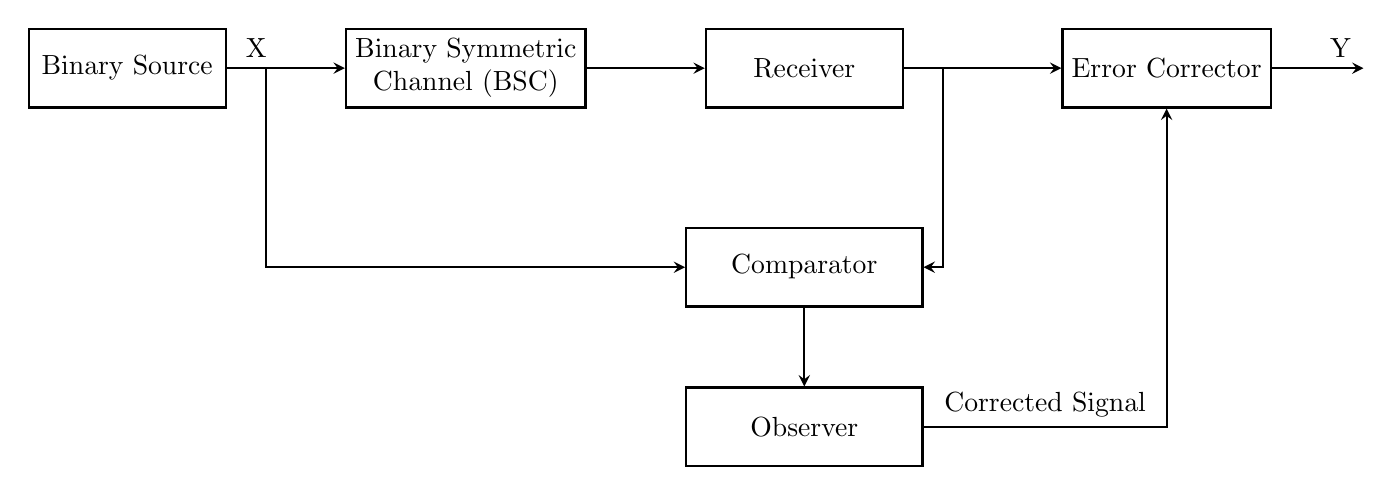
\begin{tikzpicture}[>=stealth, thick, node distance=2.5cm and 1.5cm]
    % Nodes
    \node[draw, align=center, minimum height=1cm, minimum width=2.5cm] (source) {Binary Source};
    \node[draw, align=center, minimum height=1cm, minimum width=3cm, right=of source] (bsc) {Binary Symmetric\\Channel (BSC)};
    \node[draw, align=center, minimum height=1cm, minimum width=2.5cm, right=of bsc] (receiver) {Receiver};
    \node[draw, align=center, minimum height=1cm, minimum width=2.5cm, right=2cm of receiver] (corrector) {Error Corrector};
    
    \node[draw, align=center, minimum height=1cm, minimum width=3cm, below=1.5cm of receiver] (comparator) {Comparator};
    \node[draw, align=center, minimum height=1cm, minimum width=3cm, below=1cm of comparator] (observer) {Observer};
    
    % Connections
    \draw[->] (source) -- node[above, near start] {X} (bsc);
    \draw[->] (bsc) -- (receiver);
    \draw[->] (receiver) -- (corrector);
    \draw[->] (corrector) -- node[above, near end] {Y} ++(2.5,0);

    % Feedback paths
    \draw[->] (source.east) ++(0.5,0) |- (comparator.west);
    \draw[->] (receiver.east) ++(0.5,0) |- (comparator.east);
    \draw[->] (comparator) -- (observer);
    \draw[->] (observer.east) -| node[above, near start] {Corrected Signal} (corrector.south);
\end{tikzpicture}
\caption{Binary Communication System}
\end{figure}

The binary source transmits binary data to the receiver. The comparator compares the transmitted and the received symbols. 
The comparator sends the corresponding signal to the observer. The observer, which has a noiseless channel, sends a `1` to the receiver when there is an error. 
When there is no error the observer sends a `0` to the receiver. 
Thus the observer supplies additional information to the receiver thus avoiding the noise in the channel. 
Additional information supplied by the observer is exactly equivocation of the source. 

A binary symmetric channel can be represented as: 

\begin{minipage}{.3\linewidth}
$$P(Y|X) = \begin{blockarray}{ccc}
 & 0 & 1\\
\begin{block}{c[cc]}
0 & p & q \\
1 & q & p \\
\end{block}
\end{blockarray}$$
\end{minipage}%
\hfill
\begin{minipage}{.5\linewidth}
\centering
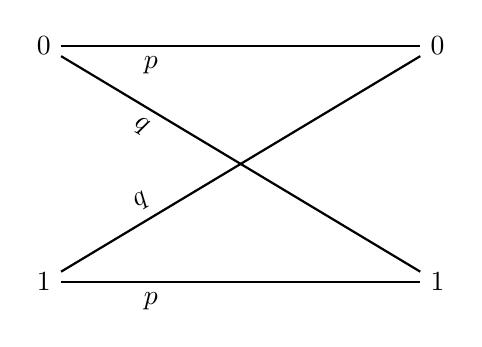
\begin{tikzpicture}[>=stealth, thick]
    % Nodes X
    \node (x1) at (0, 3) {$0$};
    \node (x2) at (0, 0) {$1$};

    % Nodes Y
    \node (y1) at (5, 3) {$0$};
    \node (y2) at (5, 0) {$1$};

    % Connections X to Y
    \draw (x1) -- node[below, near start] {$p$} (y1);
    \draw (x1) -- node[below, near start, sloped] {$q$} (y2);
    \draw (x2) -- node[above, near start, sloped] {$q$} (y1);
    \draw (x2) -- node[below, near start] {$p$} (y2);
\end{tikzpicture}
\end{minipage}

where $q = 1 - p$.

For a symmetric channel, we know that the channel capacity $C = \log_2 M - h$ here $M=2$ \& 
$$h = H(Y|X_1) = H(Y|X_2) = p \log \frac{1}{p} + q \log \frac{1}{q} = -p \log p - q \log q$$ 
\begin{align*}
C &= \log_2 M - h = \log_2 2 - (-p \log p - q \log q) \\
&= 1 + p \log p + q \log q
\end{align*} 

\subsubsection*{Problems}
\textbf{28.} Determine the channel capacity of a binary symmetrical channel whose matrix is given as 
$$P(Y|X) = \begin{bmatrix}
0.9 & 0.1 \\ 
0.1 & 0.9
\end{bmatrix}$$ 

\textbf{Ans:}
From this $p=0.9$ \& $q = 0.1$ 
\begin{align*}
C &= 1 + p \log p + q \log q \\
&= 1 + 0.9 \log_2 0.9 + 0.1 \log_2 0.1 = 1 - 0.47 = 0.53 \text{ bits/symbol}
\end{align*} 

\subsection{Binary Erasure Channel}
In communication systems, sometimes the data received may be so corrupted and thus we may not be able to judge the received output. 
Sometimes the data may be totally lost. Such a channel is called a binary erasure channel. 

A binary erasure channel can be represented as: 

\begin{minipage}{.4\linewidth}
$$P(Y|X) = \begin{blockarray}{cccc}
 & 0 & y & 1\\
\begin{block}{c[ccc]}
0 & p & 1-p & 0 \\
1 & 0 & 1-p & p \\
\end{block}
\end{blockarray}$$
\end{minipage}%
\hfill
\begin{minipage}{.5\linewidth}
\centering
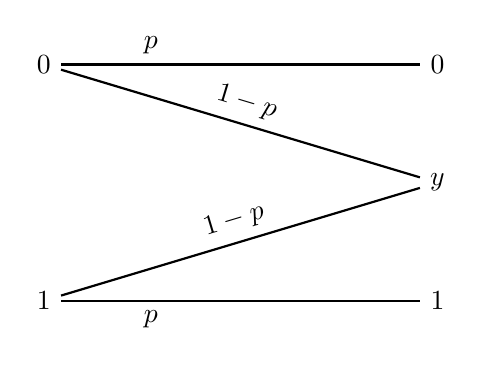
\begin{tikzpicture}[>=stealth, thick]
    % Nodes X
    \node (x1) at (0, 1.5) {$0$};
    \node (x2) at (0, -1.5) {$1$};

    % Nodes Y
    \node (y1) at (5, 1.5) {$0$};
    \node (y2) at (5, 0) {$y$};
    \node (y3) at (5, -1.5) {$1$};

    % Connections X to Y
    \draw (x1) -- node[above, near start] {$p$} (y1);
    \draw (x1) -- node[above, sloped] {$1-p$} (y2);
    \draw (x2) -- node[above, sloped] {$1-p$} (y2);
    \draw (x2) -- node[below, near start] {$p$} (y3);
\end{tikzpicture}
\end{minipage}

$$\therefore C = \max[\text{Mutual Information}] = \max[I(X,Y)] = \max[H(X) - H(X|Y)] \quad \dots \dots (1)$$ 
$$H(X) = \sum P(X)\log_2\left[\frac{1}{P(X)}\right]$$ 
Let $P(0) = \alpha$ \& $P(1) = 1-\alpha$. 
$$H(X) = \alpha \log\frac{1}{\alpha} + (1-\alpha) \log\frac{1}{1-\alpha} \quad \dots \dots (2)$$ 
$$H(X|Y) = \sum_i \sum_j P(X_i, Y_j) \log_2\left[\frac{1}{P(X_i|Y_j)}\right]$$ 

So we have to find $P(X,Y)$ \& $P(X|Y)$ 
$$P(X,Y) = P(X) \times P(Y|X) = \begin{bmatrix}
\alpha p & \alpha(1-p) & 0 \\
0 & (1-p)(1-\alpha) & (1-\alpha)p
\end{bmatrix}$$ 

$P(X|Y) = \dfrac{P(X,Y)}{P(Y)}$
\begin{align*}
P(Y_1) &= \alpha p \\
P(Y_2) &= \alpha(1-p) + (1-p)(1-\alpha) = \alpha - \alpha p + 1 - \alpha - p + \alpha p = 1-p \\
P(Y_3) &= (1-\alpha)p
\end{align*} 
$$P(X|Y) = \begin{bmatrix}
1 & \alpha & 0 \\
0 & 1-\alpha & 1
\end{bmatrix}$$ 

\begin{align*}
H(X|Y) &= \sum_i \sum_j P(X_i, Y_j)\log_2\left[\frac{1}{P(X_i|Y_j)}\right] \\
&= \alpha p \log\frac{1}{1} + \alpha(1-p)\log\frac{1}{\alpha} + (1-p)(1-\alpha)\log\frac{1}{1-\alpha} + p(1-\alpha)\log\frac{1}{1} \\
&= (1-p) \left( \alpha \log\frac{1}{\alpha} + (1-\alpha)\log\frac{1}{1-\alpha} \right) = (1-p)H(X) \quad \dots \dots (3)
\end{align*} 

Substitute 2 \& 3 in 1, we get 
$$\therefore C = \max[H(X) - (1-p)H(X)] = \max[p H(X)] = p$$ 

\subsubsection*{Problems}
\textbf{29.} Determine the channel capacity of a binary symmetrical channel whose matrix is given as 
$$P(Y|X) = \begin{bmatrix}
3/4 & 1/4 & 0 \\ 
0 & 1/4 & 3/4
\end{bmatrix}$$ 

\textbf{Ans:}
$$P(Y|X) = \begin{bmatrix}
3/4 & 1/4 & 0 \\ 
0 & 1/4 & 3/4
\end{bmatrix} \Rightarrow \begin{bmatrix}
p & 1-p & 0 \\ 
0 & 1-p & p
\end{bmatrix}$$ 
From this $p = 3/4$. 
$$C = p = 3/4 \text{ bits/symbol}$$ 

\subsection{Unsymmetric Channel}
An unsymmetric channel doesn't have any identical rows or columns. 
In this case, maximization of $H(X|Y)$ or $H(Y|X)$ possesses a problem. In such cases, maximization is obtained by using calculus of variation. 

\subsubsection{Channel Capacity of Unsymmetric Channel}
\textbf{Step 1:} The noise matrix is multiplied with a matrix of $Q_1$ and $Q_2$ which is then equated to 
$$\begin{bmatrix}
P_{11} \log P_{11} + P_{12} \log P_{12} \\ 
P_{21} \log P_{21} + P_{22} \log P_{22}
\end{bmatrix}$$ 
\textbf{Step 2:} From step 1 we obtain simultaneous equations of the variables $Q_1$ and $Q_2$ which can be solved to obtain $Q_1$ and $Q_2$. 
\textbf{Step 3:} The values of $Q_1$ and $Q_2$ are substituted in the general expression of channel capacity 
$$C = \log_2(2^{Q_1} + 2^{Q_2} + \dots + 2^{Q_n})$$ 
\subsubsection*{Problems}

\textbf{30.} Determine the channel capacity of a unsymmetric channel whose matrix is given as
$$ P(Y|X) = \begin{bmatrix} 
1/3 & 2/3 & 0 \\ 
2/3 & 1/3 & 0 \\ 
0 & 0 & 1 
\end{bmatrix} $$

\textbf{Ans:}

\textbf{Step 1:}
$$ \begin{bmatrix} 
1/3 & 2/3 & 0 \\ 
2/3 & 1/3 & 0 \\ 
0 & 0 & 1 
\end{bmatrix} 
\begin{bmatrix} Q_1 \\ Q_2 \\ Q_3 \end{bmatrix} = 
\begin{bmatrix} 
\frac{1}{3}\log_2\frac{1}{3} + \frac{2}{3}\log_2\frac{2}{3} + 0 \\ 
\frac{2}{3}\log_2\frac{2}{3} + \frac{1}{3}\log_2\frac{1}{3} + 0 \\ 
0 + 0 + 1 \log_2 1 
\end{bmatrix} $$

\textbf{Step 2:}
From these matrices, we obtain simultaneous equations:
\begin{align*}
\frac{1}{3}Q_1 + \frac{2}{3}Q_2 &= -0.92 \\
\frac{2}{3}Q_1 + \frac{1}{3}Q_2 &= -0.92
\end{align*}
Multiplying by 3:
\begin{align*}
\Rightarrow Q_1 + 2Q_2 &= -2.75 \\
2Q_1 + Q_2 &= -2.75
\end{align*}
Solving these equations:
$$ Q_1 = -0.921; \quad Q_2 = -0.917; \quad Q_3 = 0 $$

\textbf{Step 3:}
\begin{align*}
\therefore C &= \log_2(2^{Q_1} + 2^{Q_2} + 2^{Q_3}) \\
&= \log_2(2^{-0.921} + 2^{-0.917} + 2^{0}) \\
&= 1.04 \text{ bits/channel}
\end{align*}


\subsection{Binary Cascaded Channel}
Here two channels are in cascade connection.

\begin{figure}[ht]
\centering
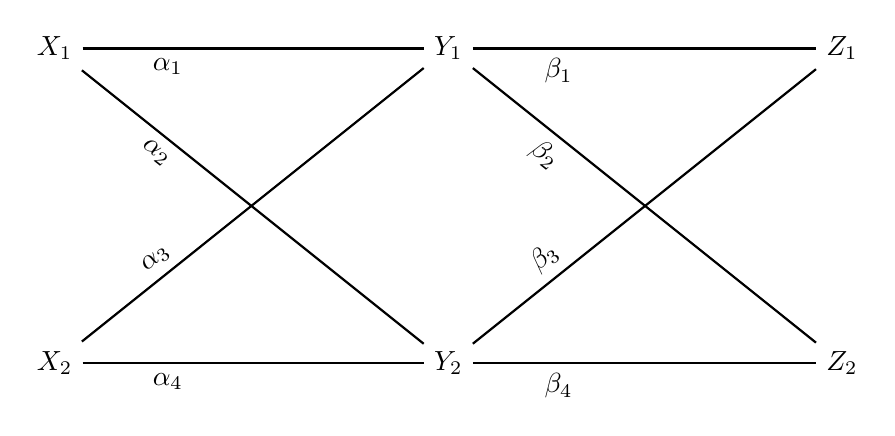
\begin{tikzpicture}[>=stealth, thick]
    % Nodes X
    \node (x1) at (0, 2) {$X_1$};
    \node (x2) at (0, -2) {$X_2$};
    
    % Nodes Y
    \node (y1) at (5, 2) {$Y_1$};
    \node (y2) at (5, -2) {$Y_2$};
    
    % Nodes Z
    \node (z1) at (10, 2) {$Z_1$};
    \node (z2) at (10, -2) {$Z_2$};
    
    % Connections X to Y
    \draw (x1) -- node[below, near start] {$\alpha_1$} (y1);
    \draw (x1) -- node[below, near start, sloped] {$\alpha_2$} (y2);
    \draw (x2) -- node[above, near start, sloped] {$\alpha_3$} (y1);
    \draw (x2) -- node[below, near start] {$\alpha_4$} (y2);
    
    % Connections Y to Z
    \draw (y1) -- node[below, near start] {$\beta_1$} (z1);
    \draw (y1) -- node[below, near start, sloped] {$\beta_2$} (z2);
    \draw (y2) -- node[above, near start, sloped] {$\beta_3$} (z1);
    \draw (y2) -- node[below, near start] {$\beta_4$} (z2);
\end{tikzpicture}
\end{figure}

$$ P(Z|X) = \begin{bmatrix} P_{11} & P_{12} \\ P_{21} & P_{22} \end{bmatrix} $$
Where,
\begin{align*}
P_{11} &= \alpha_1\beta_1 + \alpha_2\beta_3 \\
P_{12} &= \alpha_1\beta_2 + \alpha_2\beta_4 \\
P_{21} &= \alpha_3\beta_1 + \alpha_4\beta_3 \\
P_{22} &= \alpha_3\beta_2 + \alpha_4\beta_4
\end{align*}

Or equivalently:
\begin{align*}
P(Z|X) &= P(Y|X)P(Z|Y) \\
&= \begin{bmatrix}
\alpha_1 & \alpha_2 \\
\alpha_3 & \alpha_4 \\
\end{bmatrix}\begin{bmatrix}
\beta_1 & \beta_2 \\
\beta_3 & \beta_4 \\
\end{bmatrix}
\end{align*}

\subsubsection*{Problems}

\textbf{31.} Two binary symmetric channels are in cascade. Determine the channel capacity of each channel and the overall system.

\begin{figure}[ht]
\centering
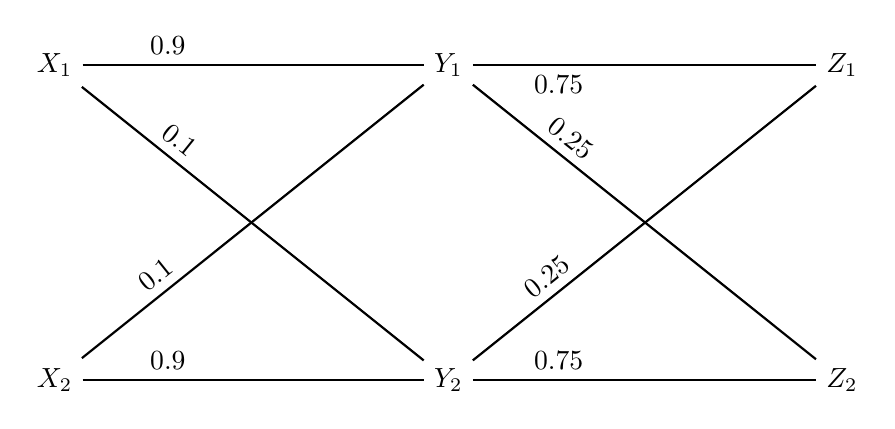
\begin{tikzpicture}[>=stealth, thick]
    % Nodes X
    \node (x1) at (0, 2) {$X_1$};
    \node (x2) at (0, -2) {$X_2$};
    
    % Nodes Y
    \node (y1) at (5, 2) {$Y_1$};
    \node (y2) at (5, -2) {$Y_2$};
    
    % Nodes Z
    \node (z1) at (10, 2) {$Z_1$};
    \node (z2) at (10, -2) {$Z_2$};
    
    % Connections X to Y
    \draw (x1) -- node[above, near start] {0.9} (y1);
    \draw (x1) -- node[above, near start, sloped] {0.1} (y2);
    \draw (x2) -- node[above, near start, sloped] {0.1} (y1);
    \draw (x2) -- node[above, near start] {0.9} (y2);
    
    % Connections Y to Z
    \draw (y1) -- node[below, near start] {0.75} (z1);
    \draw (y1) -- node[above, near start, sloped] {0.25} (z2);
    \draw (y2) -- node[above, near start, sloped] {0.25} (z1);
    \draw (y2) -- node[above, near start] {0.75} (z2);
\end{tikzpicture}
\end{figure}

\textbf{Ans:}

\textbf{$1^{st}$ Channel:}
$$ P(Y|X) = \begin{bmatrix} 0.9 & 0.1 \\ 0.1 & 0.9 \end{bmatrix} $$
Channel Capacity, $C = 1 + p \log p + q \log q$
$$ = 1 + 0.9 \log_2 0.9 + 0.1 \log_2 0.1 = 1 - 0.47 = 0.53 $$

\textbf{$2^{nd}$ Channel:}
$$ P(Z|Y) = \begin{bmatrix} 0.75 & 0.25 \\ 0.25 & 0.75 \end{bmatrix} $$
Channel Capacity, $C = 1 + p \log p + q \log q$
$$ = 1 + 0.75 \log_2 0.75 + 0.25 \log_2 0.25 = 1 - 0.81 = 0.19 $$

\textbf{Capacity of overall Channel}
$$ P(Z|X) = \begin{bmatrix} P_{11} & P_{12} \\ P_{21} & P_{22} \end{bmatrix} $$

\begin{align*}
P_{11} &= \alpha_1\beta_1 + \alpha_2\beta_3 = 0.9 \times 0.75 + 0.1 \times 0.25 = 0.7 \\
P_{12} &= \alpha_1\beta_2 + \alpha_2\beta_4 = 0.9 \times 0.25 + 0.1 \times 0.75 = 0.3 \\
P_{21} &= \alpha_3\beta_1 + \alpha_4\beta_3 = 0.1 \times 0.75 + 0.9 \times 0.25 = 0.3 \\
P_{22} &= \alpha_3\beta_2 + \alpha_4\beta_4 = 0.1 \times 0.25 + 0.9 \times 0.75 = 0.7
\end{align*}

Channel Capacity, $C = 1 + p \log p + q \log q$
$$ = 1 + 0.7 \log_2 0.7 + 0.3 \log_2 0.3 = 1 - 0.88 = 0.12 $$


\section{Capacity of A Band-Limited Gaussian Channel}
For finding the capacity of a band-limited Gaussian channel, we have to know about Shannon's theorem \& Shannon-Hartley theorem.

\subsection{Shannon's Theorem}
If there exist a source that produces 'M' number of equally likely messages generating information at the information rate 'R' with channel capacity 'C', then if $R \le C$; there exist a coding technique such that we can transmit message over the channel with minimum probability of error.

\subsubsection*{Negative Statement}
If there exist a source that produces 'M' number of equally likely messages generating information at the information rate 'R' with channel capacity 'C', then if $R > C$; there exist a coding technique such that we can transmit message over the channel with probability of error which is close to one.

\subsection{Shannon-Hartley Theorem}
Shannon-Hartley theorem is applicable to the channel affected by Gaussian noise. It states that, the channel capacity of a white, band limited Gaussian channel is
$$ C = B \log_2(1 + S/N) $$
Where,
\begin{itemize}
    \item $B$ is the channel bandwidth
    \item $S$ is the signal power
    \item $N$ is the noise power; $N = \eta B$
\end{itemize}

\subsection*{Problems}

\begin{enumerate}
    \item A voice grade channel of a telephone network has a bandwidth of 3.4 kHz.
    \begin{enumerate}
        \item Calculate the channel capacity for a SNR of 30 dB.
        \item Calculate the minimum signal to noise ratio required to support information transmitted through the telephone channel at a rate of 4800 bits per sec.
    \end{enumerate}

    \textbf{Ans:}
    \begin{enumerate}
        \item \begin{flalign*}
        \text{Given, SNR}  &= 30 \text{ dB} = 1000 && \\
        \text{Capacity }C  &= B \log_2\left(1 + \frac{S}{N}\right) && \\
        C &= 3.4 \times 10^3 \log_2(1 + 1000) && \\
        C &= 33888 \text{ bits/sec} = 33.88 \text{ kbps} && \\
        \end{flalign*}
        \item \begin{flalign*}
        \text{Given, }C &= 4.8 \text{ kbps} \quad \text{and } B = 3.4 \text{ kHz} && \\
        \therefore 4.8 \text{ kbps} &= 3.4 \text{ kHz} \cdot \log_2\left(1 + \frac{S}{N}\right) && \\
        \frac{4.8}{3.4} &= \log_2\left(1 + \frac{S}{N}\right) && \\
        1 + \frac{S}{N} &= 2^{\frac{4.8}{3.4}} \approx 2.66 && \\
        \frac{S}{N} &\approx 1.66 && \\
        \text{In dB: }\text{SNR}_{\text{dB}} &= 10 \log_{10}(1.66) \approx 2.2 \text{ dB} && \\
        \end{flalign*}
    \end{enumerate}

    \vspace{0.5cm}

    \item A communication system employs a continuous gaussian source. The channel noise is white and continuous gaussian. $B = 10 \text{ MHz}$, $SNR = 100$.
    \begin{enumerate}
        \item Find C.
        \item If SNR drops to 10, how much bandwidth is needed to achieve the same channel capacity?
        \item If B is decreased to 1 MHz, how much SNR is required to maintain the same channel capacity?
    \end{enumerate}

    \textbf{Ans:}
    \begin{enumerate}
        \item \begin{flalign*}
        C & = B \log_2\left(1 + \frac{S}{N}\right) && \\
        C & = 10 \text{ MHz} \cdot \log_2(1 + 100) && \\
        C & = 66.58 \text{ Mbps} && \\
        \end{flalign*}
        \item \begin{flalign*}
        C & = 66.58 \text{ Mbps}, \frac{S}{N} = 10 && \\
        \therefore 66.58 \text{ Mbps} & = B \cdot \log_2(1 + 10) && \\
        \Rightarrow B &= \frac{66.58 \text{ Mbps}}{\log_2(11)} = 19.24 \text{ MHz} && \\
        \end{flalign*}
        \item \begin{flalign*}
        66.58 \text{ Mbps} &= 1 \text{ MHz} \cdot \log_2\left(1 + \frac{S}{N}\right) && \\
        \frac{66.58}{1} &= \log_2\left(1 + \frac{S}{N}\right) && \\
        \Rightarrow 2^{66.58} &= 1 + \frac{S}{N} && \\
        \Rightarrow \frac{S}{N} &= 2^{66.58} - 1 \approx 2^{66.58} \approx 1.103 \times 10^{20} && \\
        \text{In dB: } 10 \log_{10}\left(2^{66.58}\right) &= 66.58 \times 10 \log_{10}(2) = 200.4 \text{ dB} && \\
        \end{flalign*}
    \end{enumerate}

    \vspace{0.5cm}

    \item Channel BW = 3.4 kHz. SNR = 20 dB. Total terminal symbols = 128 (occurring with equal probability). Successive transmission is statistically independent.
    \begin{enumerate}
        \item Calculate C.
        \item Calculate the maximum symbol rate for which error-free transmission over the channel is possible.
    \end{enumerate}

    \textbf{Ans:}
    \begin{enumerate}
        \item
        \begin{flalign*}
        \frac{S}{N} &= 20 \text{ dB} = 100 && \\
        C &= B \log_2\left(1 + \frac{S}{N}\right) && \\
        C &= 3.4 \text{ kHz} \cdot \log_2(1 + 100) && \\
        C &= 22.64 \text{ kbps}
        \end{flalign*}

        \item \begin{flalign*}
        H & = \log_2(128) = 7 \text{ bits/symbol} && \\
        R & = r \cdot H \le C && \\
        \Rightarrow r & \le \frac{C}{H} \qquad \text{(max symbol rate)} && \\
        r &\le \frac{22640 \text{ bps}}{7 \text{ bits/symbol}} && \\
        r &\le 3234 \text{ symbols/sec} && \\
        \end{flalign*}
    \end{enumerate}

\end{enumerate}

\end{document}
